\documentclass[12pt, letterpaper]{report}
\usepackage{graphicx}
\usepackage{hyperref}
\usepackage{amssymb}
\usepackage{amsmath}
\usepackage{float}
\usepackage{mathtools}
\usepackage{enumitem}
\usepackage[margin=1in]{geometry}
\usepackage[figurename=Figura]{caption}
\title{Actividad: Unidades en textos de electromagnetismo}
\author{Juan Pablo Guerrero Escudero, A01706810}
\date{3 abril, 2024}
\begin{document}
\maketitle
\subsection*{Introducción}
El objetivo de ésta actividad es investigar en diferentes libros de texto las unidades usadas, ya sea SI (sistema internacional), o 
cgs (centímetro-grado-segundo), para aprender a identificarlos y cómo cambian las fórmulas dependiendo de cada sistema. Ésto es importante 
ya que ser capaz de identificar las unidades del libro de texto consultado puede ayudar a evitar errores de cálculo y en el diseño de sistemas 
electromagnéticos.  
\subsection*{Desarrollo}
\subsubsection*{Primer libro consultado}
\begin{figure}[H]
    \centering
    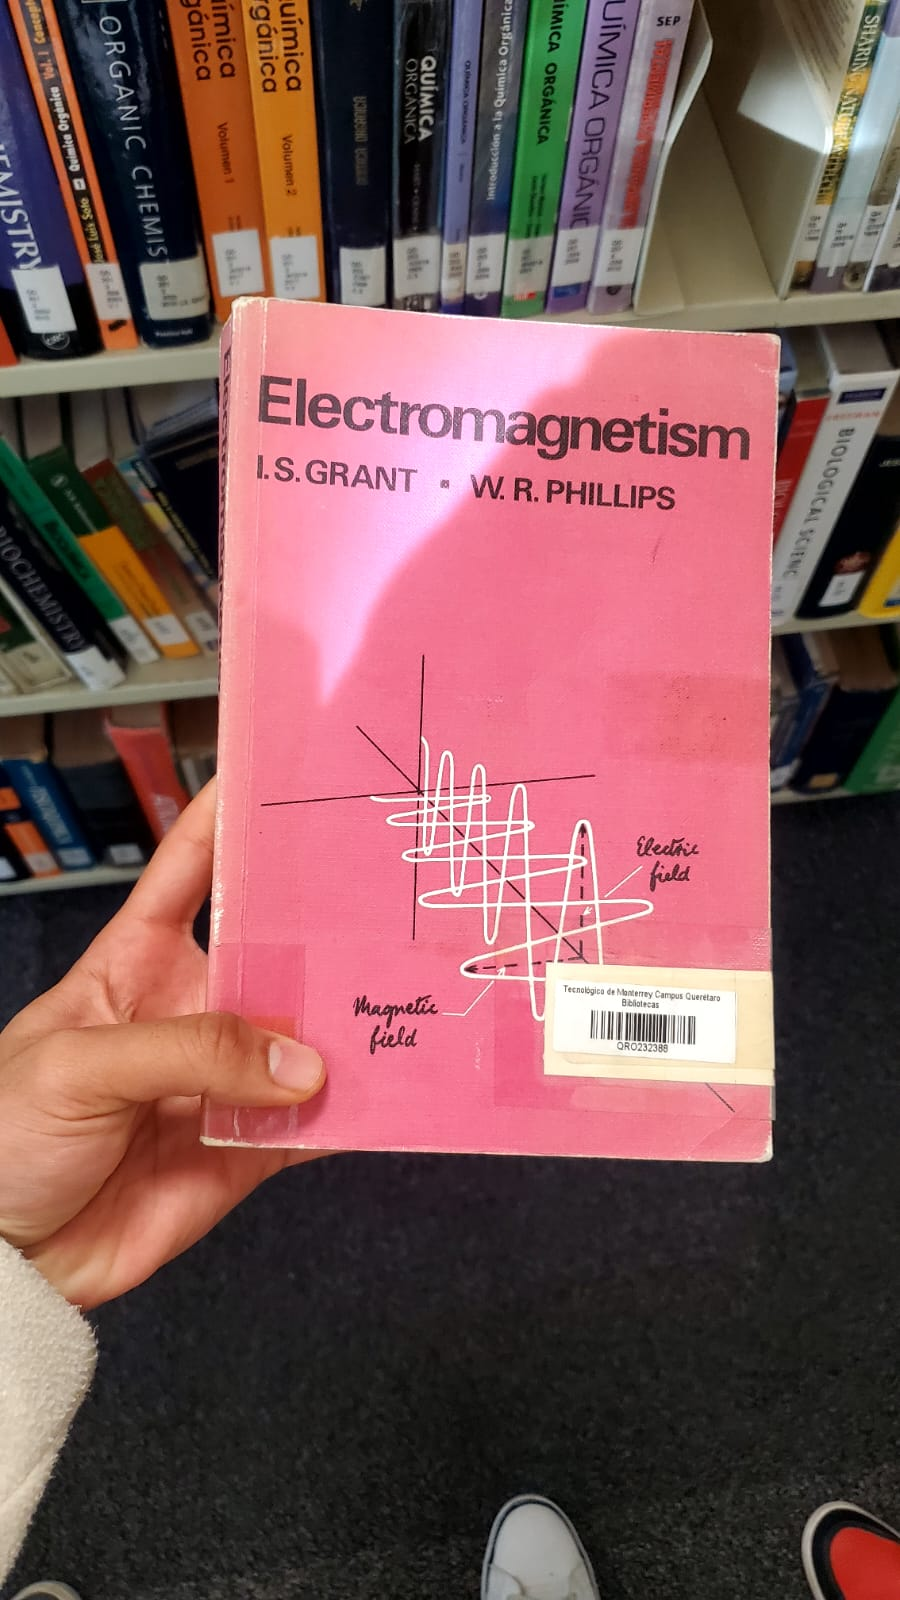
\includegraphics[height = 10cm]{2024-04-01_LibroElectromagnetismo_1.jpeg}
    \caption{Portada del primer libro consultado}
\end{figure}
El primer libro consultado es \textit{Electromagnetism} por L.S Grant, y W.R Phillips. 
El sistema que usa éste libro es SI o Sistema Internacional, menciona que ésto debido a que se consultaron 
otros textos y la mayoría ocupa SI. 
\begin{figure}[H]
    \centering
    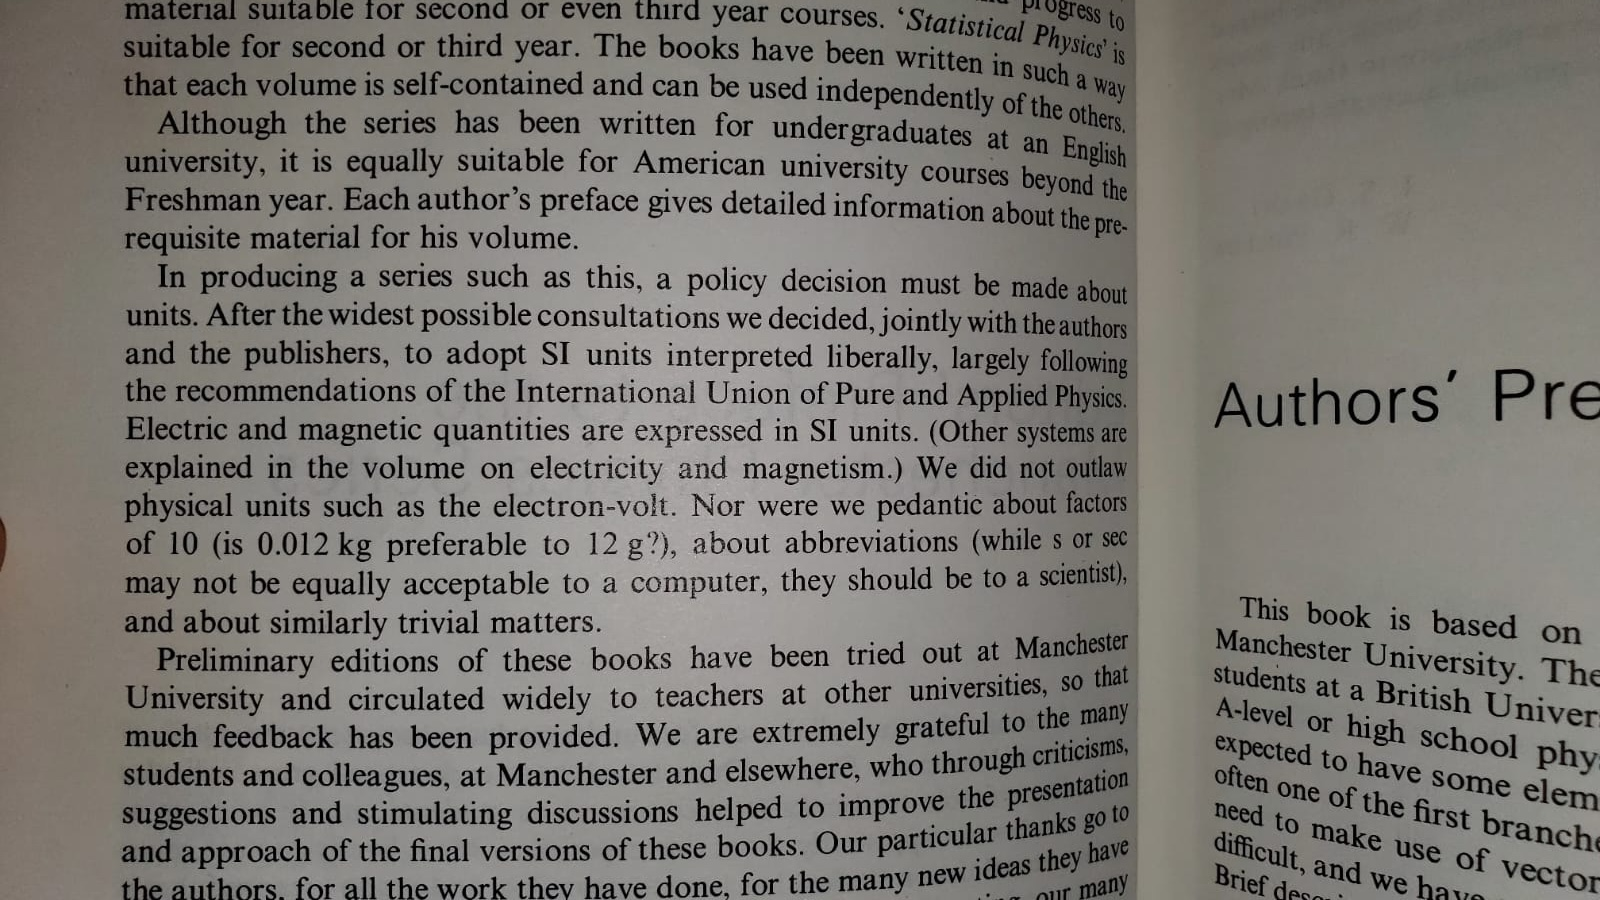
\includegraphics[height = 6cm]{2024-04-01_LibroElectromagnetismo_2.jpeg}
    \caption{Excerpto de texto mencionando el uso de SI}
\end{figure}

\subsubsection*{Segundo libro consultado}
\begin{figure}[H]
    \centering
    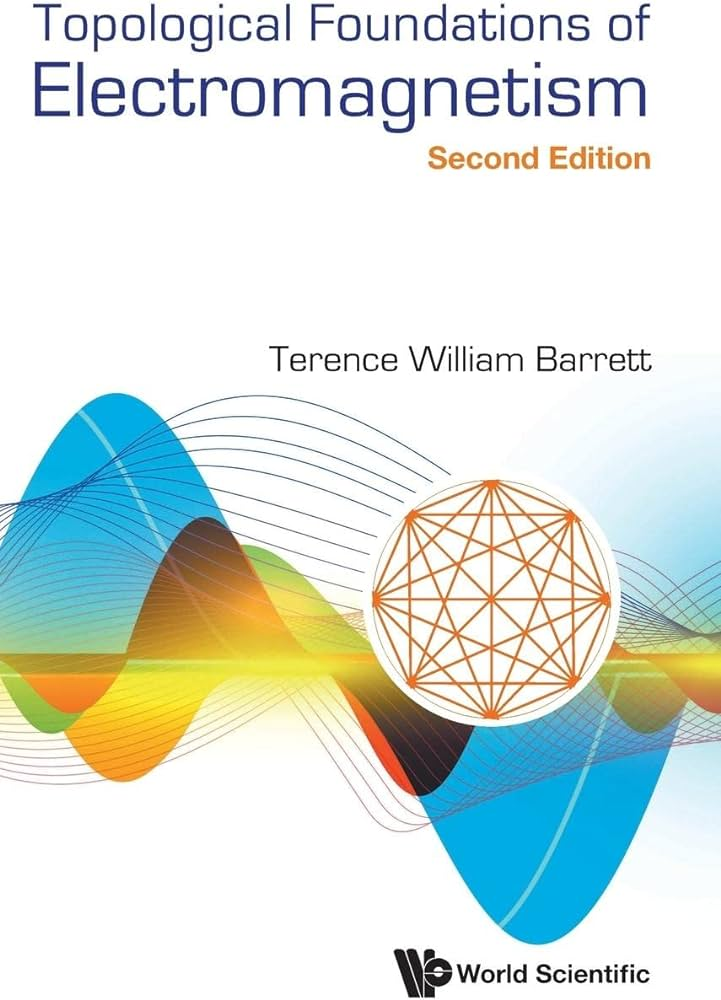
\includegraphics[height = 8cm]{2024-04-03_LibroConsultado_2.jpg}
    \caption{Libro: Topological Foundations of Electromagnetism}
\end{figure}
El segundo libro consultado es \textit{Topological Foundations of Electromagnetism} por 
Terrence William Barrett. Éste libro fue consultado electrónicamente, el cuál 
utiliza el sistema de unidades cgs (centimeter, gram, second). A continuación se muestra el fragmento de 
texto donde se menciona esto, en el pie de página: \\ 

\begin{figure}[H]
    \centering
    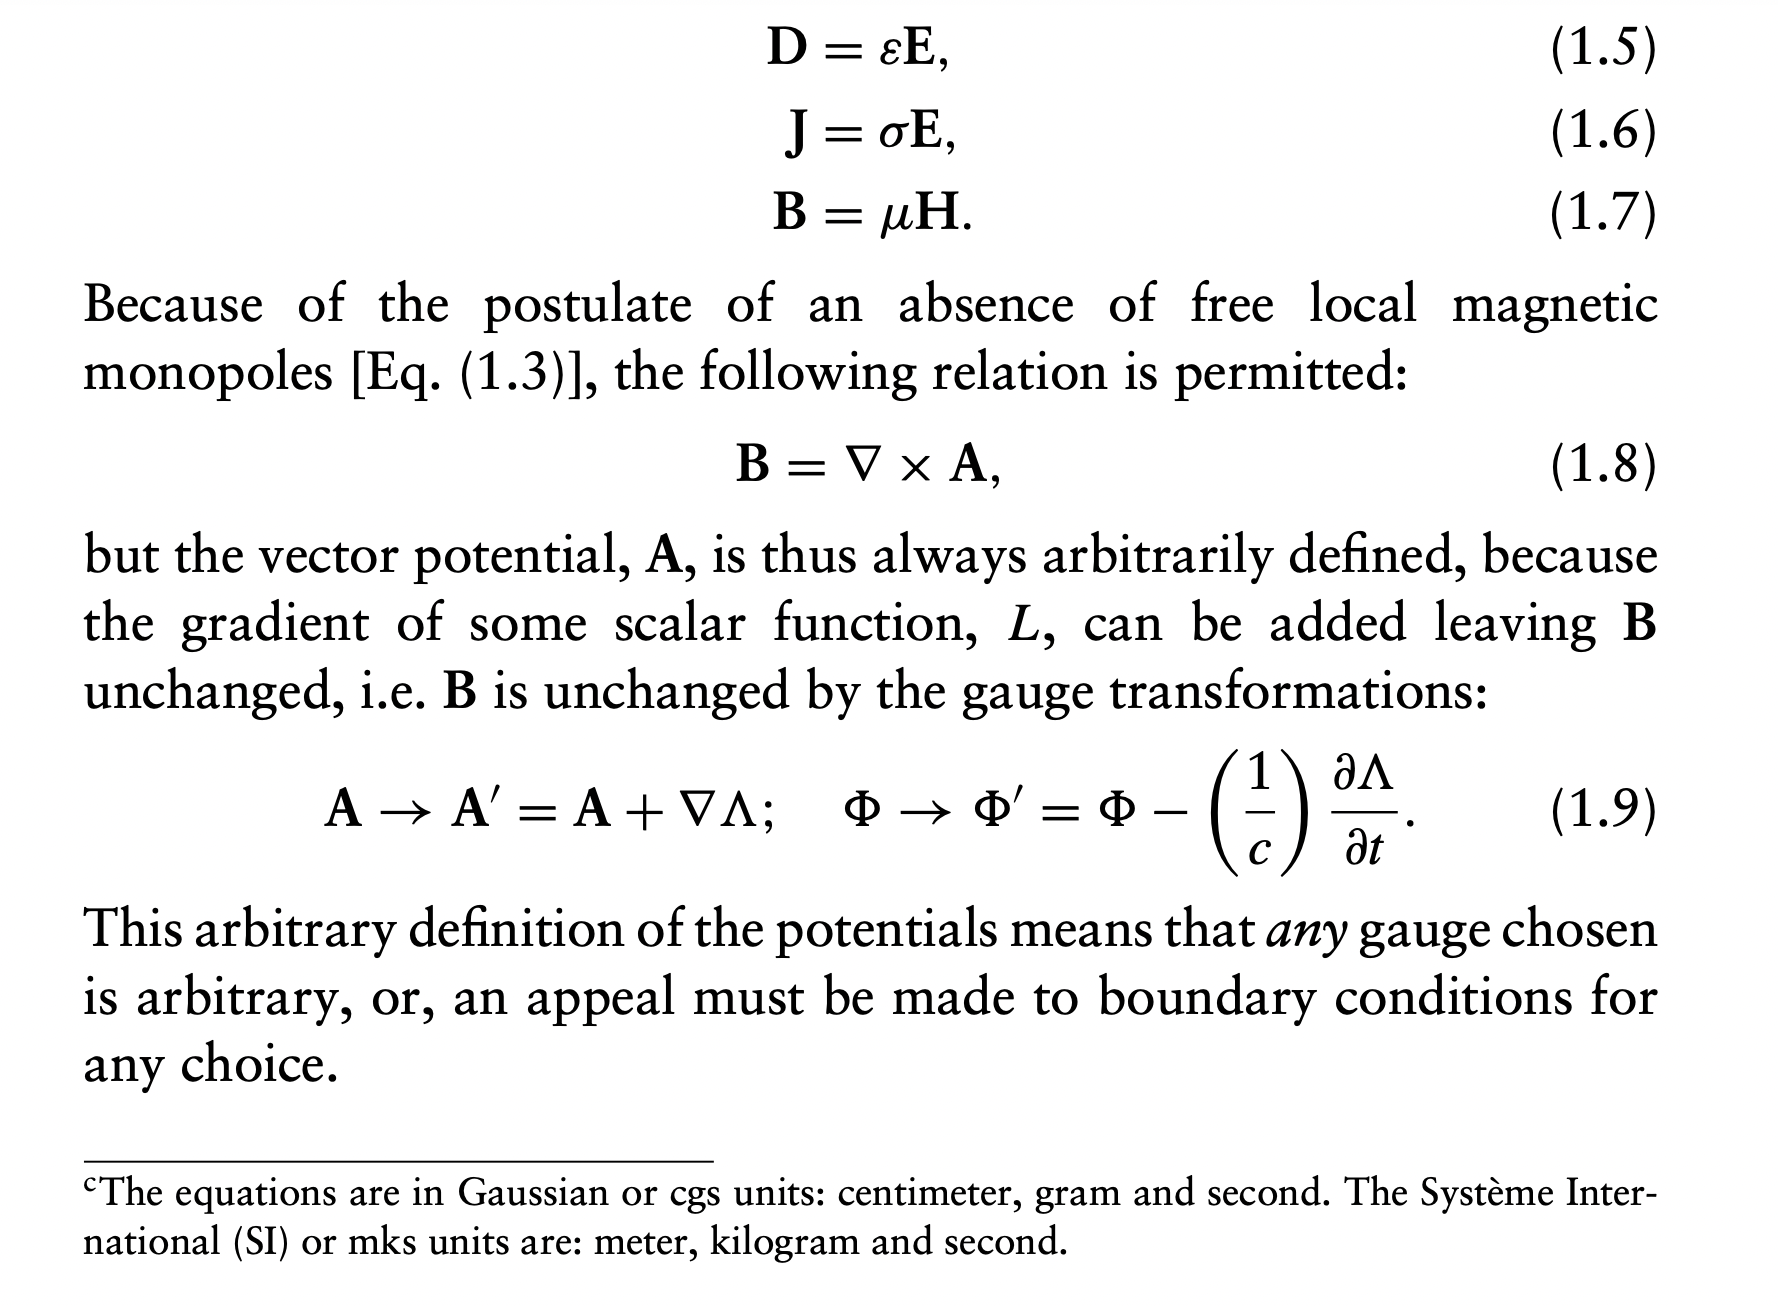
\includegraphics[height = 8cm]{2024-03-03_LibroElectromagnetismo_2_Fragmento.png}
    \caption{Fragmento del libro de texto, página 13}
\end{figure}

\subsubsection*{Reflexión Personal}
Es muy importante siempre tener presente y saber con qué unidades y sistema de unidades estás trabajando 
en algún problema o situación, ya que hacer esto puede evitar errores en el cálculo de cantidades y magnitudes, 
así como asegurarnos consistencia en nuestros procedimientos y resultados. En electromagnetismo, es importante 
porque al cambiar del SI al CGS, por ejemplo, en la fórmula de la Ley de Coulomb, en el primero se incluye una constante 
$k$, y en el segundo se omite ya que no se necesaria. \\
Por otro lado, pienso que para que un ingeniero haga un buen trabajo, debe asegurarse que las unidades son las correctas, 
ya que pueden en dado caso de omitirse, tener consecuencias tanto en el procedimiento y resultados, como en aspectos físicos 
como el cálculo de una cantidad en algún artefacto o invento. 

\subsubsection*{Referencias}
Barrett, T. W. (2008). Topological foundations of electromagnetism. In World Scientific series in contemporary chemical physics. https://doi.org/10.1142/6693\\

Grant, L. Philips, W. (1991). \textit{Electromagnetism}. Wiley. 
\end{document}